\documentclass{standalone}

\usepackage[english]{babel}
\usepackage[linesnumbered, ruled, vlined]{algorithm2e}

\usepackage{caption}

% to create listings

\usepackage{listings, lstautogobble}
\lstset{
  autogobble=true,
  frame=single,
}

\lstdefinelanguage{coq}[Objective]{Caml}{
  morekeywords={Structure, Definition, Inductive, list, return},
  sensitive=true
}

% to define font size

\usepackage{ulem}
\usepackage{moresize}
\usepackage{anyfontsize}

% to use tikz and its libraries

\usepackage{tikz-timing}
\usepackage{tikz}

\usetikzlibrary{backgrounds}
\usetikzlibrary{positioning, calc, arrows, shapes, automata, petri, patterns}

% to use tikzmark, to place and refer to marks outside the current figure

\tikzset{every picture/.style={remember picture}}

% styles for transitions

\tikzset{transition/.append style={fill=black!20, thick}}
\tikzset{transition/.append style={fill=black!20, thick}}

% styles for test and inhib arcs.

\tikzstyle{test}=[pre, *-]
\tikzstyle{inhib}=[pre, o-]

% to use colors

\usepackage{xcolor}

%%%%%%%%%%%%%%%%%%%%%%%%%%%%%%%%%%%%%%%%%%%%%%%%%%
%                  BEGIN DOCUMENT                %
%%%%%%%%%%%%%%%%%%%%%%%%%%%%%%%%%%%%%%%%%%%%%%%%%%

\begin{document}

\begin{tikzpicture}
  
  \node (abstract) [align=center, inner sep=1mm]
  {
    \begin{tabular}{@{}c@{}}
      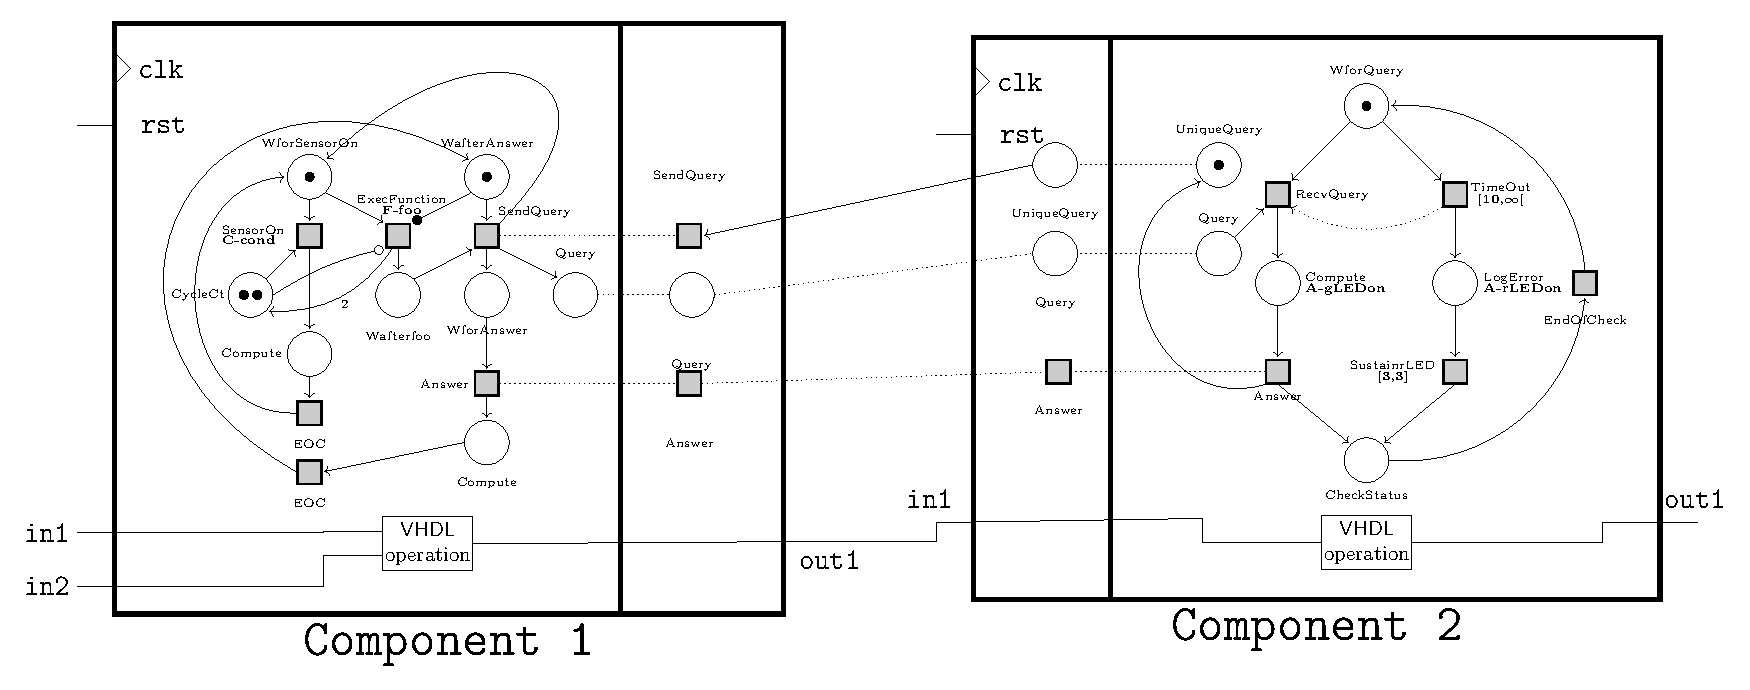
\includegraphics[keepaspectratio, width=0.1\linewidth]{abs-model}\\
      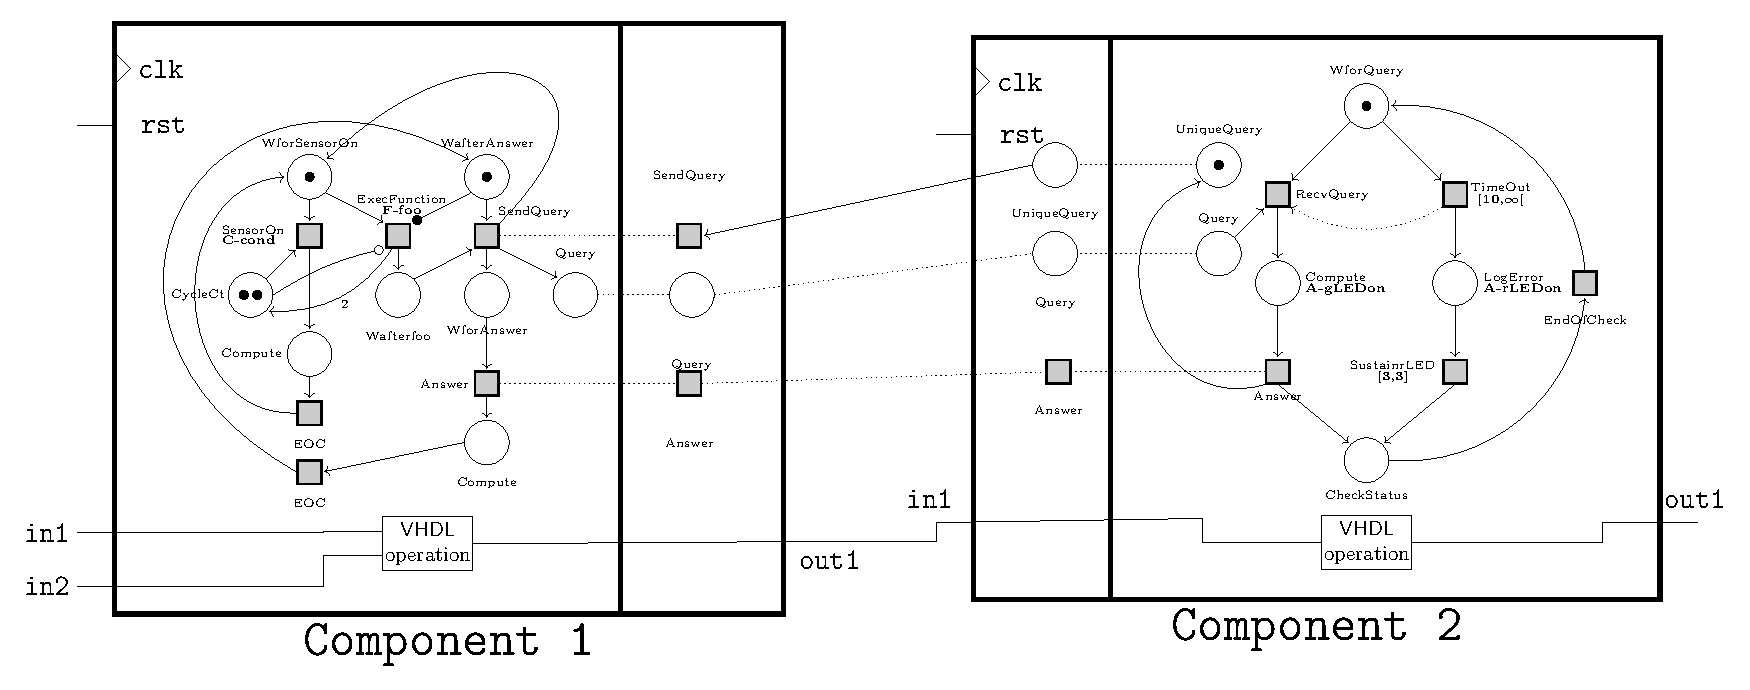
\includegraphics[keepaspectratio, width=0.1\linewidth]{abs-model}\\
    \end{tabular}

  };
  
  \node (labelabs) at ($(abstract)-(0,1)$) {
    \renewcommand{\arraystretch}{0.5}
    \begin{tabular}{c}
      \fontsize{7}{8}\selectfont Abstract\\
      \fontsize{7}{8}\selectfont model\\
      % \fontsize{7}{8}\selectfont \textcircled{1}
    \end{tabular}
  };
  \node[anchor=north, draw, circle, inner sep=.5mm] at ($(labelabs.south)$) {\fontsize{7}{8}\selectfont $1$};
  
  \draw (abstract)
  edge[loop above, looseness=8, ->]
  node{\it\bfseries \fontsize{5}{8}\selectfont designing}
  (abstract);
  
  % Implementation model node.
  
  \node (impl) at ($(abstract)+(3,0)$) [align=center, inner sep=1mm]
  {
    \begin{tabular}{@{}c@{}}
      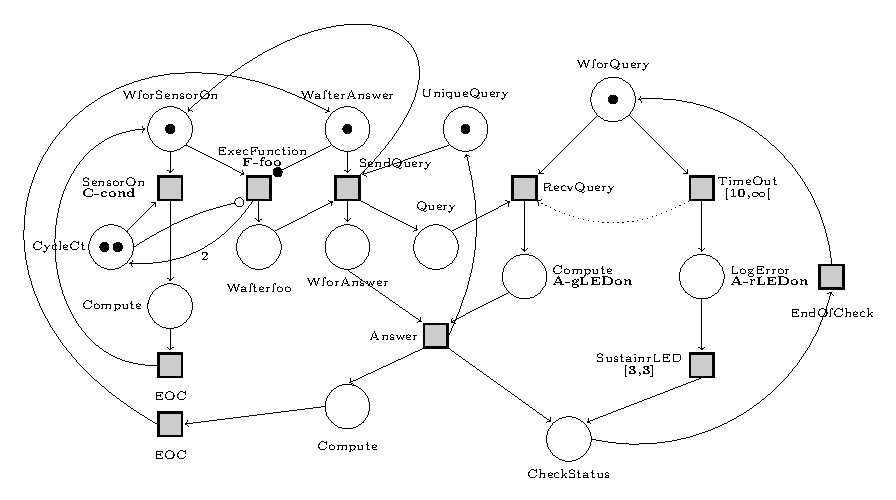
\includegraphics[keepaspectratio, width=0.1\linewidth]{impl-model}\\
      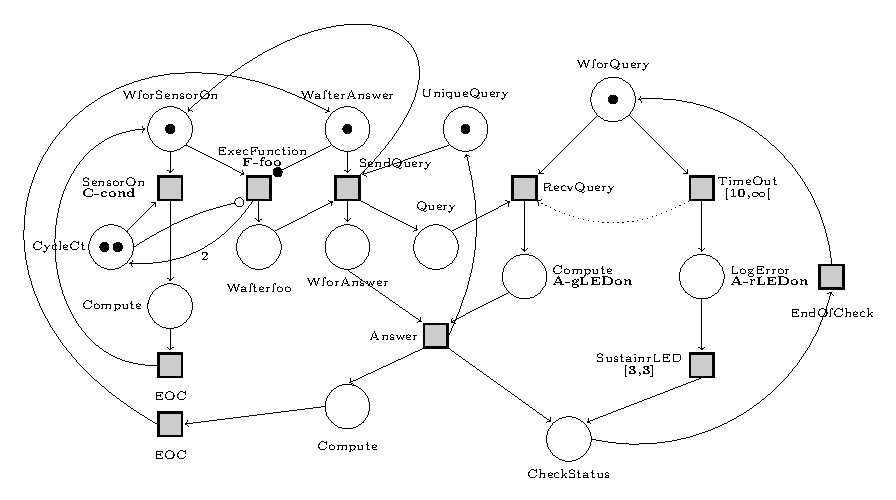
\includegraphics[keepaspectratio, width=0.1\linewidth]{impl-model}\\
    \end{tabular}

  };
  
  \draw (impl) edge[thick, <-, double]
  node[rotate=60, xshift=15pt, yshift=11pt] {
    \renewcommand{\arraystretch}{0.5}
    \begin{tabular}{c}
      \it \ssmall assembling \& \\
      \it \ssmall flattening\\
    \end{tabular}
  }  (abstract);

  \draw (impl)
  edge[loop above, looseness=11, ->]
  node{\it\bfseries \fontsize{5}{8}\selectfont analysis}
  (impl);
  
  \node (labelimpl) at ($(impl)-(0,1)$) {
    \renewcommand{\arraystretch}{0.5}
    \begin{tabular}{c}
      \fontsize{7}{8}\selectfont Implementation\\
      \fontsize{7}{8}\selectfont model\\
      % \fontsize{7}{8}\selectfont \textcircled{2}
    \end{tabular}
  };
  \node[anchor=north, draw, circle, inner sep=.5mm] at ($(labelimpl.south)$) {\fontsize{7}{8}\selectfont $2$};

  
  % Edge between impl model and abstract model.
  
  \draw ($(abstract.north east)$) edge[loop above, in=90, out=90, min distance=17mm, <-]
  node {
    \renewcommand{\arraystretch}{0.5}
    \begin{tabular}{c}
      \it \ssmall\selectfont analysis\\
      \it \ssmall\selectfont feedback\\
    \end{tabular}
  }
  ($(impl.north west)+(0,3pt)$);

  % VHDL source code node.
  
  \node (vhdl) at ($(impl)+(3,0)$) [rectangle, draw, align=center, inner
  sep=1mm] {
    \renewcommand{\arraystretch}{0.5}
    \begin{tabular}{c}
      \fontsize{7}{8}\selectfont VHDL \\
      \fontsize{7}{8}\selectfont top-level \\
      \fontsize{7}{8}\selectfont design \\
    \end{tabular}
  };
  
  \draw ($(vhdl.west)-(0.1, 0)$)
  edge[thick, <-, double]
  node[rotate=60, xshift=25pt, yshift=11pt] {
    \renewcommand{\arraystretch}{0.5}
    \begin{tabular}{c}
      \it \ssmall model-to-text \\
      \it \ssmall transformation\\
    \end{tabular}    
  }
  (impl);

  % PHYSICAL CIRCUIT
  
  \node[anchor=north, draw, circle, inner sep=.5mm] at ($(vhdl.south)-(0,.3)$) {\fontsize{7}{8}\selectfont $3$};
  
  \node (fpga) at ($(vhdl)+(3,0)$) [align=center, inner sep=1mm] {

    \tikzstyle{hpin}=[rectangle, rounded corners=0.08mm, minimum
    height=0.4mm, minimum width=1mm, fill, black, inner sep=0mm]

    \tikzstyle{vpin}=[rectangle, rounded corners=0.08mm, minimum
    height=1mm, minimum width=0.4mm, fill, black, inner sep=0mm]
    
    \begin{tikzpicture}
      \node[rectangle, rounded corners=0.4mm, inner sep=1.2mm, fill,
      black] (A) {};
      \draw[black, thick, rounded
      corners=0.1mm, line width=1mm] ($(A.north west)+(-0.06,0.06)$) rectangle
      ($(A.south east)+(0.06,-0.06)$);

      \node(pinwest0) [hpin] at ($(A.west)-(0.2, 0.04)$) {};
      \node(pinwest1) [hpin] at ($(pinwest0)+(0, 0.08)$) {};
      \node(pinwest2) [hpin] at ($(pinwest0)-(0, 0.08)$) {};
      \node(pinwest3) [hpin] at ($(pinwest1)+(0, 0.08)$) {};

      \node(pinsouth0) [vpin] at ($(A.south)-(0.04, 0.2)$) {};
      \node(pinsouth1) [vpin] at ($(pinsouth0)-(0.08, 0)$) {};
      \node(pinsouth2) [vpin] at ($(pinsouth0)+(0.08, 0)$) {};
      \node(pinsouth3) [vpin] at ($(pinsouth2)+(0.08, 0)$) {};

      \node(pineast0) [hpin] at ($(A.east)+(0.2, -0.04)$) {};
      \node(pineast1) [hpin] at ($(pineast0)+(0, 0.08)$) {};
      \node(pineast2) [hpin] at ($(pineast0)-(0, 0.08)$) {};
      \node(pineast3) [hpin] at ($(pineast1)+(0, 0.08)$) {};

      \node(pinnorth0) [vpin] at ($(A.north)+(-0.04, 0.2)$) {};
      \node(pinnorth1) [vpin] at ($(pinnorth0)-(0.08, 0)$) {};
      \node(pinnorth2) [vpin] at ($(pinnorth0)+(0.08, 0)$) {};
      \node(pinnorth3) [vpin] at ($(pinnorth2)+(0.08, 0)$) {};
      
    \end{tikzpicture}
  };
  
  \draw
  (fpga)
  edge[thick, <-, double]
  node[rotate=60, xshift=20pt, yshift=9pt] {
    \renewcommand{\arraystretch}{0.5}
    \begin{tabular}{c}
      \it \ssmall compilation/ \\
      \it \ssmall synthesis\\
    \end{tabular}    
  }
  ($(vhdl.east)+(0.1,0)$);

  \node (labelfpga) at ($(fpga)-(0,1)$) {
    \renewcommand{\arraystretch}{0.5}
    \begin{tabular}{c}
      \fontsize{7}{8}\selectfont FPGA and ASIC\\
      \fontsize{7}{8}\selectfont implementation\\
      % \fontsize{7}{8}\selectfont \textcircled{4}
    \end{tabular}
  };

  \node[anchor=north, draw, circle, inner sep=.5mm] at ($(labelfpga.south)$) {\fontsize{7}{8}\selectfont $4$};
  
  \draw[red, thick, dotted] ($(impl.north west)+(-0.35,0)$) rectangle
  ($(vhdl.south east)+(.3,-1.5)$);
  
\end{tikzpicture}

\end{document}

%%% Local Variables:
%%% mode: latex
%%% TeX-master: t
%%% End:
